\documentclass[a4paper]{article}
\usepackage[utf8x]{inputenc}
\usepackage[T1,T2A]{fontenc}
\usepackage[russian]{babel}
\usepackage{hyperref}
\usepackage{indentfirst}
\usepackage{listings}
\usepackage{color}
\usepackage{here}
\usepackage{array}
\usepackage{multirow}
\usepackage{graphicx}

\usepackage{caption}
\renewcommand{\lstlistingname}{Программа} % заголовок листингов кода

\usepackage{listings}
\lstset{ %
extendedchars=\true,
keepspaces=true,
language=bash,					% choose the language of the code
basicstyle=\footnotesize,		% the size of the fonts that are used for the code
numbers=left,					% where to put the line-numbers
numberstyle=\footnotesize,		% the size of the fonts that are used for the line-numbers
stepnumber=1,					% the step between two line-numbers. If it is 1 each line will be numbered
numbersep=5pt,					% how far the line-numbers are from the code
backgroundcolor=\color{white},	% choose the background color. You must add \usepackage{color}
showspaces=false				% show spaces adding particular underscores
showstringspaces=false,			% underline spaces within strings
showtabs=false,					% show tabs within strings adding particular underscores
frame=single,           		% adds a frame around the code
tabsize=2,						% sets default tabsize to 2 spaces
captionpos=b,					% sets the caption-position to bottom
breaklines=true,				% sets automatic line breaking
breakatwhitespace=false,		% sets if automatic breaks should only happen at whitespace
escapeinside={\%*}{*)},			% if you want to add a comment within your code
postbreak=\raisebox{0ex}[0ex][0ex]{\ensuremath{\color{red}\hookrightarrow\space}}
}

\usepackage[left=2cm,right=2cm,
top=2cm,bottom=2cm,bindingoffset=0cm]{geometry}


\begin{document}	% начало документа

\begin{titlepage}	% начало титульной страницы

	\begin{center}		% выравнивание по центру

		\large Санкт-Петербургский Политехнический Университет Петра Великого\\
		\large Институт компьютерных наук и технологий \\
		\large Кафедра компьютерных систем и программных технологий\\[6cm]
		% название института, затем отступ 6см
		
		\huge Программирование\\[0.5cm] % название работы, затем отступ 0,5см
		\large Отчет по выполнению проекта\\[0.1cm]
		\large Японская игра Сёги\\[5cm]

	\end{center}


	\begin{flushright} % выравнивание по правому краю
		\begin{minipage}{0.25\textwidth} % врезка в половину ширины текста
			\begin{flushleft} % выровнять её содержимое по левому краю

				\large\textbf{Работу выполнил:}\\
				\large Леженин Ю.И.\\
				\large {Группа:} 13501/4\\
				
				\large \textbf{Преподаватель:}\\
				\large Вылегжанина К.Д.

			\end{flushleft}
		\end{minipage}
	\end{flushright}
	
	\vfill % заполнить всё доступное ниже пространство

	\begin{center}
	\large Санкт-Петербург\\
	\large \the\year % вывести дату
	\end{center} % закончить выравнивание по центру

\thispagestyle{empty} % не нумеровать страницу
\end{titlepage} % конец титульной страницы

\vfill % заполнить всё доступное ниже пространство



% Содержание
\tableofcontents
\newpage



\section{Японская игра Сеги}

\subsection{Игровые принадлежности}

Доска сёги – 9x9 клеток, нумерующихся сверху вниз и справа налево. Клетки имеют прямоугольную форму, никак не обозначены и не имеют цвета. «Сверху» расставляются в три ряда белые фигуры – пятиугольные дощечки с обозначениями фигур. Играют два игрока. «Белые» и «черные» – это обозначение играющих, фигуры в сёги одного цвета, принадлежность последних определяется направлением острого угла дощечки. Фигура всегда устанавливается острой стороной к противнику. У каждого игрока по 20 фигур 8 наименований, отличающихся друг от друга своей ценностью, силой и рисунком ходов.

У каждой стороны есть один король, одна ладья, один слон, два золотых генерала, два серебряных генерала, два коня, два копья и девять пешек. В крайнем ряду, рядом с копьями располагаются кони. Рядом с конями – серебряные генералы. Рядом с серебряными генералами – золотые генералы. В центре, между двумя золотыми генералами находится король. На втором ряду – только две фигуры. Перед конем с левой стороны находится слон. Перед конем с правой стороны – ладья. В третьем ряду расположены девять пешек.

\subsection{Порядок игры}

Игроки делают ходы поочередно. Первые ходят чёрные. Ход представляет собой перемещение одной из фигур своего цвета, имеющихся на доске, на любое разрешенное поле согласно правилам передвижения фигур или выставление (сброс) фигуры находящейся в резерве. Фигуры «в резерве» (или по-другому «в руке») – это фигуры, взятые (сбитые) у противника.

В сёги при достижении фигурами специальной зоны (лагерь противника) они могут быть усилены (превращены). При превращении фигура переворачивается. В сёги усилиться может любая фигура кроме короля и золотого генерала.

Цель игры – поставить мат королю противника. Считается, что поставлен мат, когда король находится под ударом вражеской фигуры, т.е. находится в поле, куда может походить вражеская фигура, а возможности защититься или уйти нет.

\subsection{Взятие фигур}

«Взятие» – это ход на поле, занятое фигурой противника. В этом случае фигура противника снимается с доски и размещается рядом с ней. В отличие от шахмат, где взятые фигуры удаляются до конца игры, в сёги они могут в дальнейшем быть использованы как свои. Эти фигуры находятся в «резерве» («в руке») и в любой момент такая фигура может быть выставлена (сброшена) на любое свободное поле. 

\subsection{Ходы фигур}

\begin{itemize}
	\item Король, 
	 ходит как шахматный король — на одно поле в любом направлении.
	 
	\item Ладья, ходит как шахматная ладья — на любое количество полей по горизонтали и 	     вертикали.

	 После превращения:

     Дракон, ходит и как ладья, и как король.

	\item Слон,ходит как шахматный слон — на любое число полей по диагонали.

	 После превращения:

	 Лошадь, ходит и как слон, и как король.

	\item Золотой генерал, ходит на любое соседнее поле, кроме полей сзади по диагонали.

	\item Серебряный генерал, ходит на любое соседнее поле, кроме полей справа, слева и 	 	 снизу.

	 После превращения:

	 Перевёрнутый серебряный генера, ходит как золотой генерал.

	\item Конь, ходит буквой «Т» вперёд, то есть на два поля вперёд, и сразу на одно поле  вправо или влево. Единственная фигура сёги, которая может перескакивать через другие 		 фигуры.

	 После превращения:

     Перевёрнутый конь, ходит как золото.

	\item Копьё, ходит на любое число полей прямо вперёд. Иногда, также, называется стрела 	 или пика.

	 После переворота:

	 Перевёрнутое копьё, Ходит как золото.

    \item Пешка, ходит на одно поле прямо вперёд. Бьёт так же, как и ходит.

	 После переворота:

	 Перевёрнутая пешка, ходит как золото.
	
\end{itemize}

\subsection{Превращение}

Когда фигура достигает лагеря противника (зоны превращения) у неё возникает возможность стать превращенной (исключение составляют лишь король и золотой генерал, которые превращаться не могут). Но превращение не является обязательным, оно может быть осуществлено при любом очередном ходе (сначала передвижение, затем превращение), но только если эта фигура по-прежнему находится в лагере противника. Фигура может быть также превращена за пределами зоны превращения – в момент выхода из нее. При превращении фигура переворачивается сразу после хода и приобретает свойства превращенной фигуры. Для большинства фигур это способности золотого генерала, ладья и слон превращаются соответственно в короля-дракона и коня-дракона. Обратное превращение не допускается.

Превращение обязательно для фигур, которые не могут продолжать игру со свойствами непревращенных фигур, такие случаи возможны для пешки, копья и коня.

Если превращенная фигура взята противником, то она теряет свои способности и приобретает первоначальные свойства. Выставление

Фигура, находящаяся «в руке», может быть выставлена (сброшена) на любое свободное поле доски, что считается очередным ходом. Фигура сбрасывается только в непревращённом виде (даже если она была превращенной до взятия). Нельзя выставляться на поле занятое фигурой противника. После выставления фигура приобретает те же права, что и находящиеся на доске. Если фигура сброшена в лагерь противника, она может превратиться, только сделав следующий ход, даже если он сделан на поле за пределами зоны превращения.

\subsection{Запрещенные ходы}

Следующие ходы запрещены:

\begin{itemize}

	\item Сдваивание пешек (нифу). Когда на одной из вертикалей имеется не превращённая 		 пешка, не разрешается выставлять другую пешку на ту же вертикаль.
	
	\item Выставление пешки с матом (учи-фу-тсумэ). Не разрешается выставлять пешку с 			 матом королю противника. Однако объявлять мат очередным ходом пешки, находящейся на 		 доске, разрешено.
	
	\item Выставленние фигуры запертой. Запрещается сбрасывать фигуры таким образом, что у 	 них будет отсутствовать возможность хода в дальнейшем.
	
\end{itemize}

Игроку, сделавшему запрещенный ход, может быть присуждено поражение.

\subsection{Ничья}

Большинство партий в сёги оканчиваются либо матом, либо признанием поражения одним из игроков, однако ничья также возможна.

\begin{itemize}


	\item Повторение
	
	Пытаясь избежать проигрыша или ухудшения позиции, возможные как для одной, так и для 		другой стороны, игроки могут сознательно повторять ходы. Ничья объявляется при 				четырёхкратном повторении ситуации на доске с учетом захваченных фигур.


	\item Вечный шах

	В сёги нельзя форсировать ничью вечным шахом, как в шахматах. Если в результате серии 		шахов одного из соперников, позиция была повторена троекратно, то шахующий обязан 			изменить свой ход, иначе ему будет засчитано поражение.
   
\end{itemize}


\section{Проектирование приложения, позволяющего играть в Сёги}

\subsection{Концепция приложения} 

В ходе проектирования было разработана концепция продукта.
Созданное приложение должно предполагать возможность игры двух игроков (человека и человека или человека и компьютера) в Сёги согласно правилам перечисленнам в предыдщем разделе. Кроме того, необходимо реализовать систему сохранения и загрузки игровых партий. Также, приложение должно обладать графическим интерфейсом, позволяющим выполнять вышеперечисленные действия.

\subsection{Минимально работоспособный продукт}

Минимальноым роботоспособным продуктом было признано консольное приложение, позволяющие вести игру в Сёги двум игрокам. 

\subsection{Прецеденты использования}

На основе разработанной концепции была составлена UML диаграмма прцедентов использовани (рис.\ref{pic:use_case}).

\begin{figure}[H]
	\begin{center}
		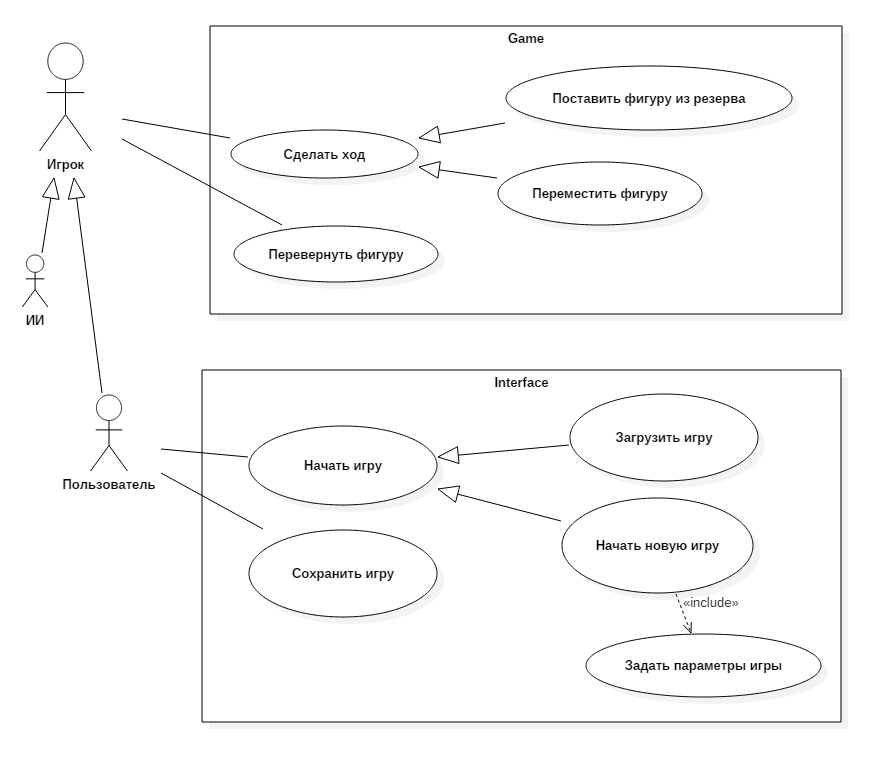
\includegraphics[scale=0.5]{../diagrams/UseCaseDiagram1.png}
		\caption{Диаграмма прцедентов использования}
		\label{pic:use_case}
	\end{center}
\end{figure}

Прецеденты были разделены на 2 части. Первая часть относиться к игровой логике, а вторая к интерфейсу приложения, взаимодействующему с пользователем.

\subsection{Основные компоненты приложения}

На основе анализа концепции и выделенных прецедентов использования было принято решение выделить три основных компонента, которые будут входить в состав продукта:

\begin{enumerate}
	\item Библиотека
	
	 Включает в себя игровую модель, а также должна обеспечивать соблюдение правил при   	 ее изменении, сообщать об игровой ситуации и опредлять моменты окончания игры. 			 Кроме того, в библиотеке должны быть реализованы простой исскуственный интелект для      	 игры в Сёги и механизм сохранения и загрузки партий. На основе этого было выделена      	 два интерфейса: первый обеспечивает доступ к игровой модели, взаимодействе с ней, а        	 второй позволяет использовать искуственный интелект для игры.

	\item Консольное приложение
	
	Должно визуализировать с помощью текста игровую модель и позволять пользоватлю 				взаимодействовать с ней, а также предоставлять возможность использовать остальные 			функциональности, поддреживаемые библиотекой.
	
	\item Графическое приложение 

	Гафически визуализирует игровую модель, предоставляет пользователю графический интерфейс для взаимодействеия с ней и выполнения остальный действий предусмотренных в реализации библиотеки. 
\end{enumerate}

\begin{figure}[H]
	\begin{center}
		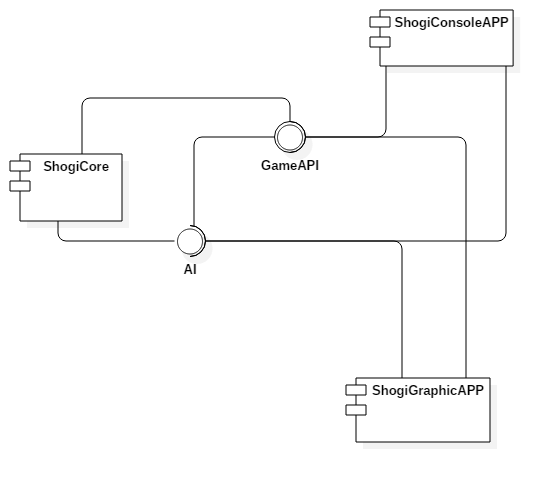
\includegraphics[scale=0.7]{../diagrams/ComponentDiagram1.png}
		\caption{Диаграмма компонентов}
		\label{pic:components}
	\end{center}
\end{figure}

Так, на рис. \ref{pic:components} изображена UML диаграмма компонентов, описывающих взаимодействие компонентов и интерфейсов.


\subsection{Генерируемые файлы и их структура}

В ходе работы приложение предполагается создавать файлы сохранения, открывать и читать их. Для того, чтобы обеспечить удобный парсинг файлов сохранения было решено использовать формат JSON. Этот формат легко читается как компьютером, так и человеком. Кроме того, существует множество готовых инструментов предназначенных для работы с JSON, которые могли бы использоваться в процессе разработки. Пример файла сохранения приведен в листинге \ref{listing:save_example}.

\captionof{lstlisting}{save\_example.json}
\label{listing:save_example} 
\lstinputlisting[label=code:hello]{../save_example.json}
\parindent=0.6cm

 Файл сохранения содержит информацию об очередности хода, список фигур на доске и их положение, а также спиок захваченных фигур.

\subsection{Используемые инструменты}

Было принято решение, для реализации приложения соответсвующего концепции ипользовать ряд сторонних интсрументов. 

\subsubsection{Qt}

Qt - кроссплатформенный инструментарий разработки ПО, помимо всего, включающий средства для теститрования (Qt Test), разработки графического интерфеса (Qt Widget) и локализации (Qt Translation), которые необходимы для реализации проекта. Также было принято решение использовать файлы ресурсов, позволяющие хранить данные, необходимые для работы приложения прямо в исполняемом файле. Именно наличие этих инструментов стало основопологающим фактором при выборе Qt. По очевидным причинам использовалась последняя версия Qt 5.6.

\subsubsection{rapidJSON}

Для работы с данными в формате JSON использовалась библиотека rapidJSON. Это библиотека состоит только из заголовочных файлов поэтому она кроссплатформена, легкопереносима и обладает небольшим объемом. Также она обладает довольно удобными для пользованиями интерфесами и предоставляет возможность проверять синтаксис JSON строк до начала разбора. Эта библиотека являет проектым с открытым кодом и активно поддерживается разработчиками, что также является не маловажным плюсом.

\section{Реализация приложения, позволяющего играть в Сёги}

\subsection{Среда разработки}

\begin{itemize}
	\item Операционная система: Windows 10
	\item Интегрирование среда разработки: CLion 2016.1.2
	\item Система автоматической сборки: Cmake 3.5.1
	\item Компилятор: GCC 4.9.3
\end{itemize}

\subsection{Реализация основных компонентов приложения}

\subsubsection{Библиотека ShogiCore}
	
	Для реализации всех запланированных функциональстей было принято решение, разделить обязанности между тремя основными интерфейсами и двумя классами:
	
	\begin{enumerate}
	\item \textbf{AbstractBoard}
	
	Данный интерфейс представляет возможность взаимодействовать с игровый модель, которая представляет собой доску с фигурами. С помощью него можно пераставлять фигуры, удалять их с доски и ставить новые. Также интерфейс позволяет получать списки захваченных фигур и фигур, находящихся в игре.  
	
	\item \textbf{AbstractGameLogic} 
	
	Интерфейс позволяющий контролировать соблюдение игровых правил и определять игровые ситуации. 
	
	\item \textbf{GameSaver} и \textbf{GameLoader}
	
	Эти классы соответсвенно ппедоставляют возможность сохранения и загрузки игры. Для выполнения данных действий классы взаимодействют с интерфесами SaveWriter и SaveReader, необходимые для записи данные в какю-либо структуру данных. Пользователь может самостоятельно создавать реализации данных интефесов, что позволяет хранить данные в любом удобным для него формате.
	
	\item \textbf{AI}
	
	Данный интерфес позволяет соверщать ходы искуственному интелекту.	
	\end{enumerate}

Все интерфесы могут быть реализованы различным образом, что позволяет легко изменять и улучшать отдельные части библиотеки независимо от остальных.

Также в библиотеке существуют класс \textbf{ShogiGame}, реализующий основной API, основная задача которого заключается в орагнизации работы классов, реализующих все вышеперчисленные интерфейсы.	
	
\subsubsection{Консольное приложение}

Консольное приложение было условно поделено на сцены. Для каждой сцены был создан класс, в котором реализованно вывод необходимой информации и взаимодействие с пользователем. Также был создан класс \textbf{Application}, в котором была, реализвана логика переключения между сценами.

TODO скрины 

\subsubsection{Графическое приложение}

Консольное приложение было реализована с помощью интсрументов Qt. С помощью Qt Widgets было созданы классыд двух основных окон \textbf{MenuWindow} и \textbf{GameWindow}, которые отвечали за основное меню и окно с игрой соответсвенно. Было выделен виджет \textbf{GameGraphicFrame}, который отвечал за отрисовку игровой модели и обработку нажатий кнопок мыши. В нем была инкапсулирована вся логика взаимодействия с библиотекой. Данный виджет стал часть окна \textbf{GameWindow}.
   
\section{Процесс обеспечения качества и тестирование}

В процессе разработки приложения для обеспечения качества были использованы различные интсрументы.

\subsection{Теститрование}

В ходе разработки проекта регулярно проводилось автомотическое тестирование. Для этого использовался инстрмент Qt Test, который упрощает написание тестирующего кода, а также предоставляет информацию о результатах теститрования в удобном виде, что позволяет систиматезировать. В ходе разработки был написан функциональный тест, с помощью которого выполнялась проверка работоспособности основных функциональстей библиотеки. Также был реализован модульный тест, позволяющий проверять выполнение задач, за которые отвечали отдельны классы.

Тестирование позволило обеспечить работоспособность продукта в ходе всего процесса разработки, а также сильно упрощало поиск допущенных ошибок и обеспечивало их своевременное исправление.   

\subsection{Статический и динамический анализ}

Для улучшения качества и надежности создаваемого продукта использовались средства для статического и динамического анализа кода.

Для статического анализа использовалась программа Cppcheck v1.72. Данный инструмент производит анализ кода до момента компиляции и способен обнаруживать ряд ошибок связанных со стилем кода, его переносимостью и производительностью конечного продукта. Использование данной программы позволило создавать качественный код с высокой скоростью работы.

Для динамического анализа использовалась программа Valgrind v3.10.1, которая производит анализ во время работы приложения и позволяет определить места утечки памяти и обнаружить ошибки, связанные с неправильным обращением к ней. Применение данного инструмента позволило создать надежное приложение и обеспечить правильное взаимодействие с оперативной памяью устройства, на котором оно будет запущено.

\subsection{Непрерывная интеграция}

В ходе разработки активно использовалась среда непрерывной интеграции под название Jenkins, чья суть в том, что при каждом обновления репозитория производилась полная сборка проекта, его теститрование, статический и динамический анализ, а также собиралась различная статистическа информация типа количества строк кода и количества пометок "TODO". После выполнения описанного цикла полученная информация обрабатовалась и визуализровалась с помощтю графиков и таблиц. Это позволило облегчить процесс разработки приложения, но и в то же время повысить качество создаваемого продукта. Также благодаря этой среде была получена возможность контролировать процесс написания кода, что положительно сказалось на конечном результате.

\subsection{Просмотр кода}

Активно применялась практика так называемого "code review", суть которого заключается в том, что достаточно квалифицированные люди просматривали код, в создании которого они не участвовали, и высказывали свои замечения и предложения. Так в ходе разработки было проведено 3 просмотра, нацеленных на выявление ошибок и недоработок, связанных  непосредственно с кодом и его стилем, и 1 просмотр, целью которого было выявление ошибок в проектировании архитектуры приложения. В ходе данных проверок было получено в общей сложности больше 100 замечений, которые были в итоге исправлены, что позволило значительно качество и надежность кода.   

\subsection{Демонтрации}

Во время создания приложения было проведено 4 демонстрации, на которых группой людей, представляющих собой потенциальных пользовоталей разработываемого приложения, были сделаны различные замечания и высказаны множество предложений и пожеланий, основанных на внешнем виде продукта и стандартном цикле работы с ним. Анализ полученной информации позволял обнаруживать недочеты присутсвующие в продукте на том, или ином этапе разработки, а также определять дальнейшие направления улучшения и расширения проекта, что, безусловно, положительно сказалось на конечном результате.

\section{Выводы}

\section{Приложение 1}

\section{Приложение 2}

%\subsection{Листинг}
%
%\captionof{lstlisting}{hell\_o.c} % для печати символ '_' требует выходной символ '\'
%\lstinputlisting[label=code:hello]{listings/hell_o.c}
%\parindent=1cm % командна \lstinputlisting сбивает параментры отступа
%Текст без отступа (следует за вставкой)
%
%Новый параграф
%
%\noindent Новый параграф с принудительно выключенным отступом
%
%
%\subsection{Частичный листинг}
%% настрока частичного ввода (требуется один раз)
%\makeatletter
%\def\lst@PlaceNumber{\llap{\normalfont
%                \lst@numberstyle{\the\lst@lineno}\kern\lst@numbersep}}
%\makeatother
%
%\captionof{lstlisting}{фрагмент hell\_o.c}
%\lstinputlisting[label=code:hello_mod, linerange={4-5}]{listings/hell_o.c}
%\parindent=1cm
%
%\subsection{Таблица}
%
%\begin{table}[H]
%	\begin{center}
%		\begin{tabular}{|l|l|}
%			\hline
%			top left & top right\\ \hline
%			bot left & bot right\\ \hline
%		\end{tabular}
%		\caption{ Название таблицы}
%		\label{tabular:tab_examp}
%	\end{center}
%\end{table}
%
\end{document}